\documentclass{llncs}
\usepackage{fullpage}
\usepackage{float}
\usepackage{tikz}
\usepackage{amsmath}
\usetikzlibrary{arrows}

\usepackage{enumitem}
\usepackage{graphicx}
\usepackage{array}
\usepackage{pgfgantt}
\usepackage{booktabs}
\usepackage[utf8]{inputenc}

% Redefine las subsecciones para usar letras en lugar de números
\usepackage{titlesec}
\renewcommand\thesubsection{\alph{subsection})}

\begin{document}

\title{Planificación de tareas}

\author{Miguel Ángel Dorado Maldonado}
\institute{\email{miguelangeldorado10@uma.es} \\
TCIS. Universidad de Málaga.}

\maketitle 

\vspace{1cm} 

\section{Un proyecto viene especificado por el siguiente orden de precedencia de sus actividades:}

\begin{align*}
B &\longrightarrow C \\
A, B &\longrightarrow D \\
C, D &\longrightarrow E \\
A, B &\longrightarrow F \\
F &\longrightarrow G \\
E, G &\longrightarrow H \\
H &\longrightarrow I \\
\end{align*}

\begin{enumerate}

	\item[a)] Realice un diagrama con la programación de las actividades.

		\begin{figure}[H]
		\centering
		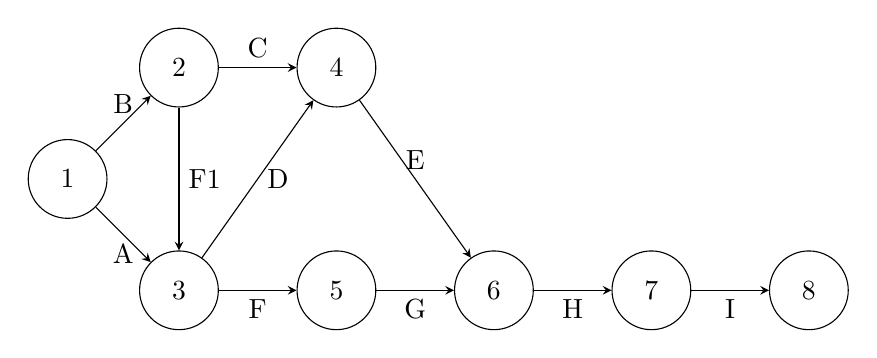
\begin{tikzpicture}[->, >=stealth, node distance=2cm, state/.style={circle, draw, minimum size=1cm}]

		\node[state] (1) {1};
		\node[state] (2) [above right of=1] {2};
		\node[state] (3) [below right of=1] {3};
		\node[state] (4) [right of=2] {4};
		\node[state] (5) [right of=3] {5};
		\node[state] (6) [right of=5] {6};
		\node[state] (7) [right of=6] {7};
		\node[state] (8) [right of=7] {8};

		\path 
		(1) edge node[above] {B} (2)
				edge node[below] {A} (3)
		(2) edge node[above] {C} (4)
				edge node[right] {F1} (3)
		(3) edge node[below] {F} (5)
		 		edge node[right] {D} (4)
		(4)	edge node[above] {E} (6)
		(5) edge node[below] {G} (6)
		(6) edge node[below] {H} (7)
		(7) edge node[below] {I} (8);

		\end{tikzpicture}
		\caption{Diagrama de precedencia de actividades}
		\end{figure}

	\item[b)] Suponga el siguiente cuadro de duraciones para cada actividad.

		\begin{center}
		\begin{tabular}{|c|ccccccccc|}
			\hline
			$Actividad$ & $A$ & $B$ & $C$ & $D$ & $E$ & $F$ & $G$ & $H$ & $I$ \\
			\hline
			Duración (días) & 3 & 1 & 2 & 1 & 10 & 2 & 8 & 6 & 3 \\
			\hline
		\end{tabular}
		\end{center}
		Determine la duración del proyecto y su camino crítico.

				\begin{figure}[H]
					\centering
						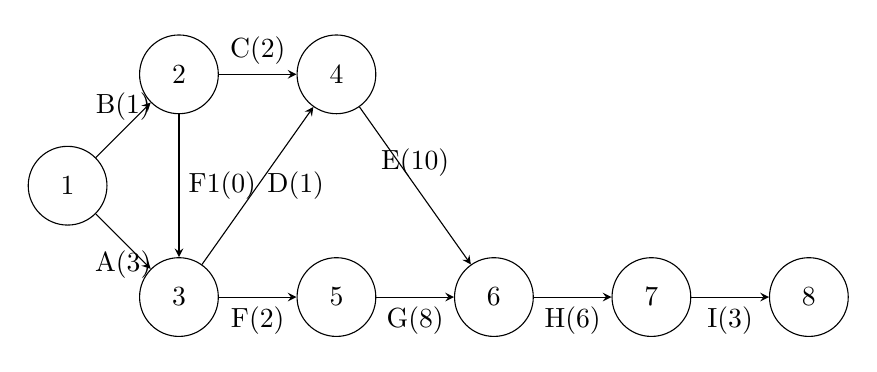
\begin{tikzpicture}[->, >=stealth, node distance=2cm, state/.style={circle, draw, minimum size=1cm}]

							\node[state] (1) {1};
							\node[state] (2) [above right of=1] {2};
							\node[state] (3) [below right of=1] {3};
							\node[state] (4) [right of=2] {4};
							\node[state] (5) [right of=3] {5};
							\node[state] (6) [right of=5] {6};
							\node[state] (7) [right of=6] {7};
							\node[state] (8) [right of=7] {8};

							\path 
							(1) edge node[above] {B(1)} (2)
									edge node[below] {A(3)} (3)
							(2) edge node[above] {C(2)} (4)
									edge node[right] {F1(0)} (3)
							(3) edge node[below] {F(2)} (5)
									edge node[right] {D(1)} (4)
							(4)	edge node[above] {E(10)} (6)
							(5) edge node[below] {G(8)} (6)
							(6) edge node[below] {H(6)} (7)
							(7) edge node[below] {I(3)} (8);

						\end{tikzpicture}
					\caption{Diagrama de precedencia de actividades con duración}
				\end{figure}

				Conocidos los tiempos de duración de cada actividad, se calcula el camino crítico y la duración del proyecto por el método CPM. Para ello se calculan los tiempos de inicio early ($E_i$) y late ($L_i$) de cada actividad.

				\begin{center}
					\begin{tabular}{|@{\hspace{0.3cm}}c@{\hspace{0.3cm}}|@{\hspace{0.3cm}}c@{\hspace{0.3cm}}|@{\hspace{0.3cm}}c@{\hspace{0.3cm}}|}
						\hline
						$t$ & $E_i$ & $L_i$ \\
						\hline
						1 & 0 & 0 \\
						2 & 1 & 2 \\
						3 & 3 & 3 \\
						4 & 4 & 4 \\
						5 & 5 & 6 \\
						6 & 14 & 14 \\
						7 & 20 & 20 \\
						8 & 23 & 23 \\
						\hline
					\end{tabular}
				\end{center}


				Una vez calculados estos tiempos, es necesario obtener los tiempos de holgura para encontrar el camino crítico. La holgura ($H_{ij}$) se calcula como $L_j$ - $E_i$ - $D_{ij}$, donde $L_j$ es el tiempo de terminación más tardío de la actividad, $E_i$ es el tiempo de inicio más temprano de la actividad y $D_{ij}$ es la duración de la actividad. $R_{ij}$ representa los nodos que representan inicio y fin de la actividad.

				\begin{center}
					\begin{tabular}{|c|c|c|c|c|c|c|}
						\hline
						Tarea & $R_{ij}$ & $D_{ij}$ & $E_i$ & $L_j$ & $H_{ij}$ & Crítico\\
						A & $1\longrightarrow 3$ & 3 & 0 & 3 & 0 & X \\
						B & $1\longrightarrow 2$ & 1 & 0 & 2 & 1 & \\
						C & $2\longrightarrow 4$ & 2 & 1 & 4 & 1 & \\
						D & $3\longrightarrow 4$ & 1 & 3 & 4 & 0 & X \\
						E & $4\longrightarrow 6$ & 10 & 4 & 14 & 0 & X \\
						F & $3\longrightarrow 5$ & 2 & 3 & 6 & 1 &  \\
						G & $5\longrightarrow 6$ & 8 & 5 & 14 & 1 &  \\
						H & $6\longrightarrow 7$ & 6 & 14 & 20 & 0 & X \\
						I & $7\longrightarrow 8$ & 3 & 20 & 23 & 0 & X \\
						\hline
					\end{tabular}
				\end{center}

				De esta forma se obtiene que el camino crítico es aquel cuyos valores de holgura sea 0. Por tanto, el camino crítico es $A \longrightarrow D \longrightarrow E \longrightarrow H \longrightarrow I$ y la duración del proyecto es de 23 días.

	\newpage
	\item[c)] Obtenga el diagrama de Gantt.

		\begin{ganttchart}[
    hgrid,
    vgrid,
    title label font=\bfseries\footnotesize,
    title label node/.append style={below=-1ex},
    include title in canvas=false,
    bar label font=\footnotesize,
    bar height=0.6,
    x unit=0.5cm,
    y unit chart=0.8cm
]{1}{28} 
    \gantttitle{Semana 1}{7}
    \gantttitle{Semana 2}{7}
    \gantttitle{Semana 3}{7}
    \gantttitle{Semana 4}{7} \\
		\ganttbar[bar/.style={fill=red!70}]{A}{1}{3} \\
		\ganttbar[bar/.style={fill=green!70}]{B}{1}{1} \\
		\ganttbar[bar/.style={fill=green!70}]{C}{2}{3} \\
		\ganttbar[bar/.style={fill=red!70}]{D}{4}{4} \\
		\ganttbar[bar/.style={fill=red!70}]{E}{5}{14} \\
		\ganttbar[bar/.style={fill=green!70}]{F}{4}{5} \\
		\ganttbar[bar/.style={fill=green!70}]{G}{6}{13} \\
		\ganttbar[bar/.style={fill=red!70}]{H}{15}{20} \\
		\ganttbar[bar/.style={fill=red!70}]{I}{21}{23}
		\ganttlink{elem0}{elem3}
		\ganttlink{elem3}{elem4}
		\ganttlink{elem4}{elem7}
		\ganttlink{elem7}{elem8}
		\ganttlink{elem1}{elem2}
		\ganttlink{elem1}{elem2}
		\ganttlink{elem1}{elem3}
		\ganttlink{elem2}{elem4}
		\ganttlink{elem0}{elem5}
		\ganttlink{elem1}{elem5}
		\ganttlink{elem5}{elem6}
		\ganttlink{elem6}{elem7}

	\end{ganttchart}
	\begin{center}
	
\begin{tikzpicture}
			\draw[fill=red!70] (0,0) rectangle ++(0.4,0.4);
			\node[right=0.5cm of {(0.4,0)}] {Tarea crítica};
			\draw[fill=green!70] (8,0) rectangle ++(0.4,0.4);
			\node[right=0.5cm of {(8.4,0)}] {Tarea con holgura};
	\end{tikzpicture}
	\end{center}
\end{enumerate}

\section{Considere el proyecto que viene determinado por el siguiente diagrama con la programación de sus actividades.}

\begin{figure}[H]
	\begin{center}
		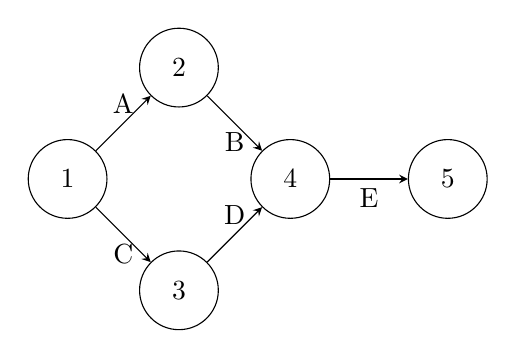
\begin{tikzpicture}[->, >=stealth, node distance=2cm, state/.style={circle, draw, minimum size=1cm}]

		\node[state] (1) {1};
		\node[state] (2) [above right of=1] {2};
		\node[state] (3) [below right of=1] {3};
		\node[state] (4) [below right of=2] {4};
		\node[state] (5) [right of=4] {5};

		\path 
		(1) edge node[above] {A} (2)
				edge node[below] {C} (3)
		(2) edge node[below] {B} (4)
		(3) edge node[above] {D} (4)
		(4) edge node[below] {E} (5);

		\end{tikzpicture}
	\end{center}
\end{figure}


\begin{enumerate}
	\item[a)] Suponga el siguiente cuadro de duraciones para cada actividad.

		\begin{center}
			\begin{tabular}{|c|ccccc|}
				\hline
				$Actividad$ & $A$ & $B$ & $C$ & $D$ & $E$ \\
				\hline
				Duración (días) & 3 & 4 & 2 & 6 & 3 \\
				\hline
			\end{tabular}
		\end{center}


	\item[b)] Suponga que no se conoce la duración de las actividades de forma determinista pero se estiman los siguientes tiempos optimista ($t_o$), más probable ($t_m$) y pesimista ($t_p$).

		\begin{center}
			\begin{tabular}{|c|c@{\hspace{0.3cm}}c@{\hspace{0.3cm}}c|}
					\hline
					$Actividad$ & $t_o$ & $t_m$ & $t_p$ \\
					\hline
					A & 2 & 5 & 8 \\
					B & 1 & 4 & 6 \\
					C & 2 & 2 & 3 \\
					D & 4 & 6 & 9 \\
					E & 3 & 5 & 7 \\
					\hline
			\end{tabular}
	\end{center}

	Determine la duración estimada del proyecto y su varianza, así como su camino crítico.

\end{enumerate}

\section{La realización de un proyecto viene especificado por el siguiente orden de las actividades:}

	\begin{align*}
		A &\longrightarrow C \\
		B, C &\longrightarrow E \\
		D &\longrightarrow F \\
	\end{align*}
La duración de las actividades no se conoce de forma determinista pero se estiman los siguientes tiempos optimista, medio y pesimista. Determine la duración estimada del proyecto y su varianza.

\begin{center}
	\begin{tabular}{|c|c@{\hspace{0.3cm}}c@{\hspace{0.3cm}}c|}
		\hline
		$Actividad$ & $t_o$ & $t_m$ & $t_p$ \\
		\hline
		A & 3 & 5 & 10 \\
		B & 2 & 4 & 6 \\
		C & 2 & 2 & 2 \\
		D & 4 & 7 & 9 \\
		E & 4 & 5 & 7 \\
		F & 3 & 6 & 10 \\
		\hline
	\end{tabular}
\end{center}
	

\end{document}

